
Sukurtas įrankis, turi daug funkcionalumų. Gali automatiškai arba rankiniu būdu išgauti duomenis iš daugelio mobiliųjų įrenginių.  Įrankis tinkamas telefonams su ekrano užraktu bei be ekrano užrakto. Įrankis gali ištraukti duomenis iš „Android“ įrenginio „userdata“ particijos atvaizdo, bei gauti juos iš įrenginio, kuris jau paleistas „TWRP“ režime.  Darbo eigoje sukurtas įrankis gali taip pat ištraukti ir apdoroti SMS, kontaktų, skambučių, bei naršyklės duomenų bazes. Taip apdorota medžiaga gali būti panaudota teisminei ekspertizei. Skriptas turi daug informacinių dialogų, kurie leidžia vartotojui lengvai suprasti kas vyksta ir kokius žingsnius reikia įvykdyti, kad duomenų išgavimas vyktų sklandžiai.

Įrankis veikia su daugeliu Samsung įrenginių, bei su kitais įrenginiais, kuriems turime galimybę suteikti „root“ teises arba įrašyti neoficialų atstatymo režimą. 

Darbo metu atliktame tyrime panaudotas įrankis sėkmingai ištraukia duomenis iš „Samsung Galaxy S5“ (veikiančio su naujausia jam prieinama „Android 6.0.1“ versiją) bei  „Samsung Galaxy S3 NEO“ (veikiančiu su naujausia jam prieinama „Android 4.4.4“ versiją). Iš šių mobiliūjų įrenginių pavyko išgauti visus analizei vertingus failus, o prireikus, tolimesnei analizei, įrankis suteikia galimybę sumontuoti atvaizdą ir atlikti analizę rankiniu būdu, analizuojant kitų programėlių duomenų bazes. 

Įrankis ne tik išgauna duomenis, bet ir juos tinkamai suformatuoja, į lengvai skaitomus tekstinius failus. Šis funkcionalumas leidžia žmonėms kurie niekada nedirbo su duomenų bazių analize lengvai peržiūrėti duomenis, tokius kaip SMS žinutes sudėliotas chronologiškai pagal gavėją, naršomų internetinių puslapių istoriją su naršymo datomis, bei URL adresais. 

Kadangi tai tik pirma pabaigta įrankio versija, jo automatinė duomenų išgavimo procedūra ribota veikti su Samsung įrenginiais. Atsižvelgiant į tai jog Lietuvoje pirmauja Samsung gamybos įrenginiai, sukurtas įrankis gali būti vertingas teisminėms analizėms. Remiantis Statcounter statistika \cite{StatcounterLithuania} (14 pav.),  virš trečdalis Lietuvoje naudojamų įrenginių yra Samsung gamybos.
\begin{figure} [h]
    \centering
    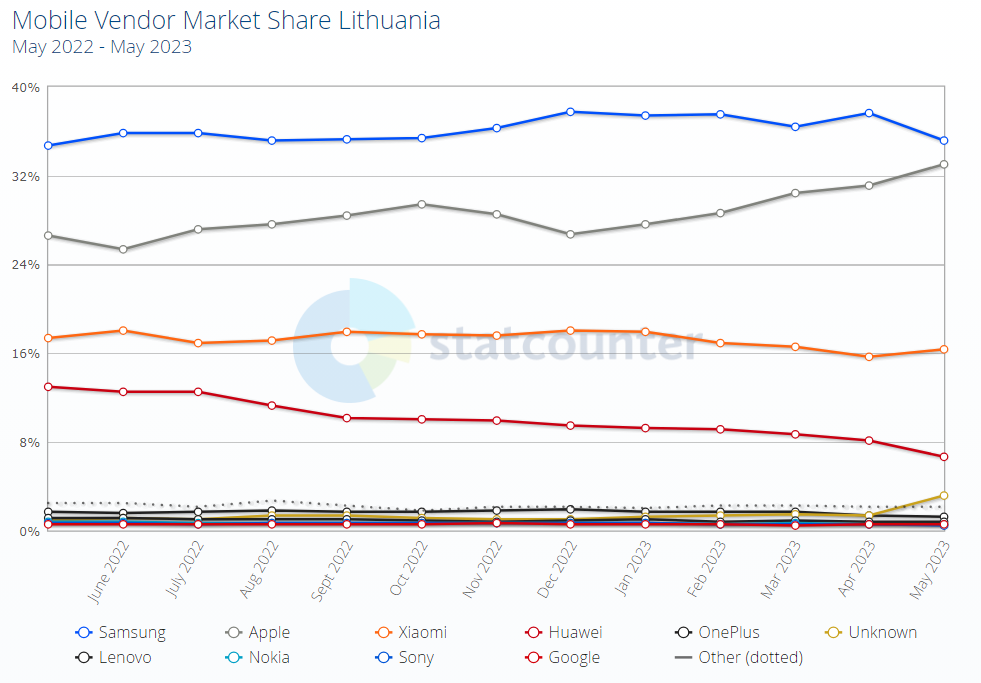
\includegraphics[width=0.85\linewidth]{stat_lt2.png}
    \caption{Mobiliųjų įrenginių pasiskirstymas pagal gamintojus Lietuvoje}
    \label{fig:LT_tel_statistics}
\end{figure}